\begin{frame}
  \begin{center}
    {\color{Maroon}\Huge Tackling New Languages}
  \end{center}
\end{frame}

\begin{frame}{Tackling New Languages}{Outline}
  \begin{enumerate}
  \item IARPA Babel
  \item Audio Keyword Search
  \item What Language Characteristics Matter?
    \begin{itemize}
    \item Morphology and vocabulary growth
    \item Writing system
    \item Tonal languages
    \item Amount of available training data
    \end{itemize}
  \item A Recipe for a New Language
    \begin{itemize}
    \item Pronunciations
    \item Flat-start Initialization
    \item Multilingual Features
    \item Web Text
    \end{itemize}
  \end{enumerate}
\end{frame}

\begin{frame}{The IARPA Babel Program}{}
  \Large{``\ldots to \alert{rapidly develop} speech recognition
    capability for keyword search in a previously unstudied
    language, working with speech recorded in a variety of
    conditions with limited amounts of transcription.''}\par
\end{frame}

\begin{frame}{Rapid Development}{Time allowed for surprise language model building}
  \begin{center}
    \begin{tabular}{@{}cl@{}} \toprule
      {\bf Period} & \multicolumn{1}{c}{\bf Time} \\ \midrule
      1 & 4 weeks \\
      2 & 3 weeks \\
      3 & 2 weeks \\
      4 & 1 week  \\ \bottomrule
    \end{tabular}
  \end{center}
\end{frame}

\begin{frame}{The IARPA Babel Program}{}
  \Large{``\ldots to rapidly develop speech recognition
    capability for keyword search in a \alert{previously unstudied
      language}, working with speech recorded in a variety of
    conditions with limited amounts of transcription.''}\par
\end{frame}

\begin{frame}{Babel Languages}{}
  \begin{center}
    \begin{tabular}{@{}llll@{}} \toprule
      \multicolumn{1}{c}{\bf Period 1} & \multicolumn{1}{c}{\bf Period 2} & \multicolumn{1}{c}{\bf Period 3} & \multicolumn{1}{c}{\bf Period 4} \\ \midrule
      Cantonese  & Assamese       & Kurmanji Kurdish & Pashto \\
      Pashto     & Bengali        & Tok Pisin        & Guaran\'{i} \\
      Turkish    & Haitian Creole & Cebuano          & Igbo \\
      Tagalog    & Lao            & Kazakh           & Amharic \\
      Vietnamese & Zulu           & Telugu           & Mongolian \\
                 & Tamil          & Lithuanian       & Javanese \\
                 &                & Swahili          & Dholuo \\
                 &                &                  & Georgian \\ \bottomrule
    \end{tabular}
  \end{center}
  \vfill
  \nb{These will be available from the LDC at \$US 25.00 per language for non-members.}
\end{frame}

\begin{frame}{The IARPA Babel Program}{}
  \Large{``\ldots to rapidly develop speech recognition
    capability for keyword search in a previously unstudied
    language, working with speech recorded in a variety of
    conditions with \alert{limited amounts of transcription}.''}\par
\end{frame}

\begin{frame}{Limited resources}{Hours of transcribed training data}
  \settowidth{\colA}{100}
  \begin{center}
    \begin{tabular}{@{}cc@{}} \toprule
      {\bf Period} & {\bf Hours} \\ \midrule
      1 & 100 \\
      2 & \aln{\colA}{r}{10} \\
      3 & \aln{\colA}{r}{3}  \\
      4 & \aln{\colA}{r}{40} \\ \bottomrule
    \end{tabular}
  \end{center}
  \vfill
  \nb{In Periods 3 and 4, no phonetic lexicons.}
\end{frame}

\begin{frame}{The IARPA Babel Program}{}
  \Large{``\ldots to rapidly develop speech recognition
    capability for \alert{keyword search} in a previously unstudied
    language, working with speech recorded in a variety of
    conditions with limited amounts of transcription.''}\par
\end{frame}

\begin{frame}{What is keyword search, and why focus on it?}{}
  {\bf Detection task}: given
    \begin{itemize}
    \item a word or short phrase and
    \item a collection of speech data,
    \end{itemize}
    \alert{where} does it occur, and \alert{how confident} are you?
    \vfill
    We can build \alert{practical} keyword search from
    \alert{unreliable} speech recognition.
\end{frame}

%% WFST search:  index generation (token and phonetic)
\begin{frame}{Building an index}{1. Generate a lattice for each segment in the collection.}
  \begin{center}
    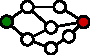
\includegraphics[width=36mm]{figures/lattice}
  \end{center}
  \begin{overlayarea}{\textwidth}{24mm}
    \begin{columns}[t]
      \column{54mm}
      \onslide<1>{
        \centerline{\bf Lattice}
        \begin{description}
        \item[Nodes] times
        \item[Edges] words (or phones) and posterior probabilities
        \end{description}
      }
      \column{54mm}
      \onslide<2>{
        \centerline{\bf Transducer}
        \begin{description}
        \item[Inputs] words (or phones)
        \item[Outputs] times
        \item[Costs] negative log-posteriors
        \end{description}
      }
    \end{columns}
  \end{overlayarea}
\end{frame}

\begin{frame}{Building an index}{2. Produce the factor automaton for each segment.}
  \begin{center}
    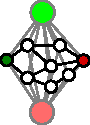
\includegraphics[width=36mm]{figures/factor}
    \end{center}
  \vfill
  Added edges have $\epsilon$ inputs, $\epsilon$ outputs, and no costs.
\end{frame}

\begin{frame}{Building an index}{3. Connect all the factor automata in parallel.}
  \begin{center}
    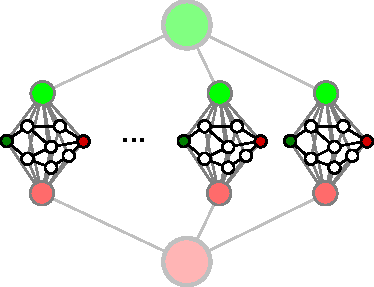
\includegraphics[width=66mm]{figures/index}
    \end{center}
  \vfill
  Added edges from start have $\epsilon$ inputs, segment ID outputs, and no costs.
  Added edges to end have $\epsilon$ inputs, $\epsilon$ outputs, and no costs.
\end{frame}

%% WFST search:  query generation / search via composition
%% 1. Query -> phone FSA
%% 2. Composition with confusability model and pruning
%% 3. (Optional) Project back to words
%% 4. Search is then simple composition with the index

%% TWV metric and its quirks

%% What Language Characteristics Matter?
%% Morphology and vocabulary growth
%% Writing system
%% Tonal languages
%% Amount of available training data
%%   multilingual feature front-ends
%%   multilingual AMs
%%   Data augmentation
%%   Semi-supervised training

%% A Recipe for a New Language (do a VLLP and a recent FLP?)
%% Pronunciations
%% Flat-start Initialization
%% Multilingual Features
%% Web Text

%% \begin{frame}{}{}
%% \end{frame}
